\documentclass{article}

% packages
\usepackage{amsmath, amsthm, thmtools, amsfonts, amssymb, luacode, catchfile, tikzducks, hyperref, ifthen}
\ifcsname c@kobocompile\endcsname
	\usepackage[a5paper, total={1072pt, 1448pt}, margin=10pt, includeheadfoot]{geometry} % set page margins
\else
	\usepackage[a4paper, margin=50pt, includeheadfoot]{geometry}
\fi
\usepackage[shortlabels]{enumitem}
\usepackage[skip=3pt, indent=0pt]{parskip}

% language
\usepackage[bidi=basic, layout=tabular, provide=*]{babel}
\ifcsname c@english\endcsname
	\babelprovide[main, import]{english}
\else
	\babelprovide[main, import]{hebrew}
	\babelprovide{rl}
\fi
%\babelfont{rm}{Libertinus Serif}
\babelfont{rm}[Renderer=Harfbuzz]{Libertinus Serif}
\babelfont{sf}{Libertinus Sans}
\babelfont{tt}{Libertinus Mono}

% style
\AddToHook{cmd/section/before}{\clearpage}	% Add line break before section
\linespread{1.3}
\setcounter{secnumdepth}{0}		% Remove default number tags from sections, this won't do well with theorems
\AtBeginDocument{\setlength{\belowdisplayskip}{3pt}}
\AtBeginDocument{\setlength{\abovedisplayskip}{3pt}}
\graphicspath{ {../images/} }

% operators
\DeclareMathOperator\cis{cis}
\DeclareMathOperator\Sp{Sp}
\DeclareMathOperator\tr{tr}
\DeclareMathOperator\im{Im}
\DeclareMathOperator\re{Re}
\DeclareMathOperator\diag{diag}
\DeclareMathOperator*\lowlim{\underline{lim}}
\DeclareMathOperator*\uplim{\overline{lim}}
\DeclareMathOperator\rng{rng}
\DeclareMathOperator\Sym{Sym}
\DeclareMathOperator\Arg{Arg}
\DeclareMathOperator\Log{Log}
\DeclareMathOperator\dom{dom}
\DeclareMathOperator\supp{Supp}
\DeclareMathOperator\var{Var}
\DeclareMathOperator\cov{Cov}

% commands
%\renewcommand\qedsymbol{\textbf{מש''ל}}
%\renewcommand\qedsymbol{\fbox{\emoji{lizard}}}
\newcommand{\Aa}[0]{\mathcal{A}}
\newcommand{\Bb}[0]{\mathcal{B}}
\newcommand{\CC}[0]{\mathbb{C}}
\newcommand{\Cc}[0]{\mathcal{C}}
\newcommand{\EE}[0]{\mathbb{E}}
\newcommand{\FF}[0]{\mathbb{F}}
\newcommand{\Ff}[0]{\mathcal{F}}
\newcommand{\Ii}[0]{\mathcal{I}}
\newcommand{\Gg}[0]{\mathcal{G}}
\newcommand{\Ll}[0]{\mathcal{L}}
\newcommand{\Mm}[0]{\mathcal{M}}
\newcommand{\NN}[0]{\mathbb{N}}
\newcommand{\Nn}[0]{\mathcal{N}}
\newcommand{\PP}[0]{\mathbb{P}}
\newcommand{\Pp}[0]{\mathcal{P}}
\newcommand{\QQ}[0]{\mathbb{Q}}
\newcommand{\RR}[0]{\mathbb{R}}
\newcommand{\Rr}[0]{\mathcal{R}}
\newcommand{\Ss}[0]{\mathcal{S}}
\newcommand{\TT}[0]{\mathbb{T}}
\newcommand{\Uu}[0]{\mathcal{U}}
\newcommand{\Vv}[0]{\mathcal{V}}
\newcommand{\Ww}[0]{\mathcal{W}}
\newcommand{\ZZ}[0]{\mathbb{Z}}
\newcommand{\acts}[0]{\circlearrowright}
\newcommand{\explain}[2] {
	\begin{flalign*}
		 && \text{#2} && \text{#1}
	\end{flalign*}
}
\newcommand{\maketitleprint}[0]{ \begin{center}
	%\begin{tikzpicture}[scale=3]
	%	\duck[graduate=gray!20!black, tassel=red!70!black]
	%\end{tikzpicture}	
	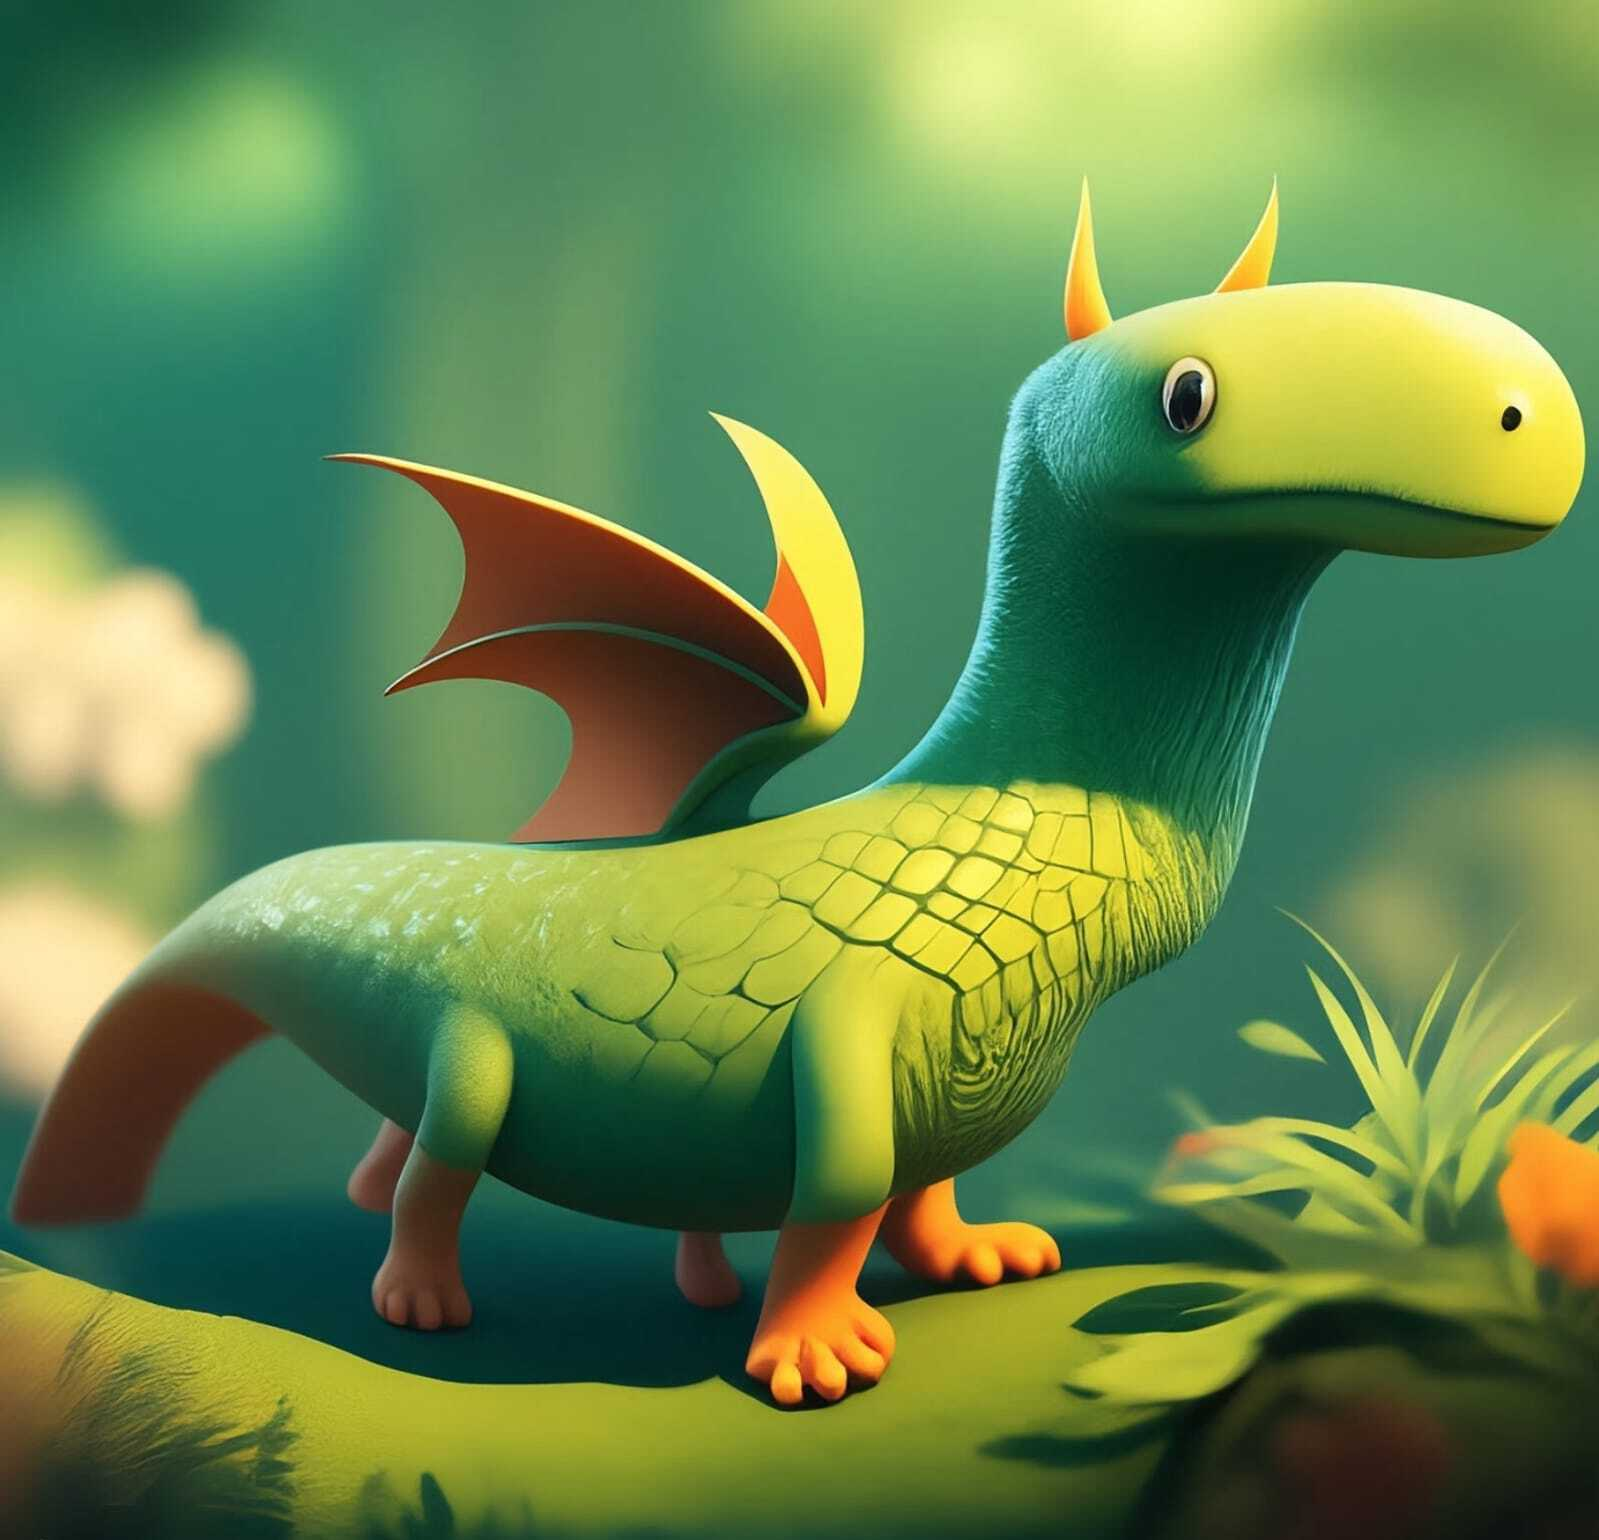
\includegraphics[width=6cm]{cover}
\end{center}
}

% theorem commands
\newtheoremstyle{c_remark}
	{}	% Space above
	{}	% Space below
	{}% Body font
	{}	% Indent amount
	{\bfseries}	% Theorem head font
	{}	% Punctuation after theorem head
	{.5em}	% Space after theorem head
	{\thmname{#1}\thmnumber{ #2}\thmnote{ \normalfont{\text{(#3)}}}}	% head content
\newtheoremstyle{c_definition}
	{3pt}	% Space above
	{3pt}	% Space below
	{}% Body font
	{}	% Indent amount
	{\bfseries}	% Theorem head font
	{}	% Punctuation after theorem head
	{.5em}	% Space after theorem head
	{\thmname{#1}\thmnumber{ #2}\thmnote{ \normalfont{\text{(#3)}}}}	% head content
\newtheoremstyle{c_plain}
	{3pt}	% Space above
	{3pt}	% Space below
	{\itshape}% Body font
	{}	% Indent amount
	{\bfseries}	% Theorem head font
	{}	% Punctuation after theorem head
	{.5em}	% Space after theorem head
	{\thmname{#1}\thmnumber{ #2}\thmnote{ \text{(#3)}}}	% head content

\ifcsname c@english\endcsname
	\theoremstyle{plain}
	\newtheorem{theorem}{Theorem}[section]
	\newtheorem{lemma}[theorem]{Lemma}
	\newtheorem{proposition}[theorem]{Proposition}
	\newtheorem*{proposition*}{Proposition}
	%\newtheorem{corollary}[theorem]{אין חלופה עברית}

	\theoremstyle{definition}
	\newtheorem{definition}[theorem]{Definition}
	\newtheorem*{definition*}{Definition}
	\newtheorem{example}{Example}[section]
	\newtheorem{exercise}{Exercise}[section]

	\theoremstyle{remark}
	\newtheorem*{remark}{Remark}
	\newtheorem*{solution}{Solution}
	\newtheorem{conclusion}[theorem]{Conclusion}
	\newtheorem{notation}[theorem]{Notation}
\else
	\theoremstyle{c_plain}
	\newtheorem{theorem}{משפט}[section]
	\newtheorem{lemma}[theorem]{למה}
	\newtheorem{proposition}[theorem]{טענה}
	\newtheorem*{proposition*}{טענה}
	%\newtheorem{corollary}[theorem]{אין חלופה עברית}

	\theoremstyle{c_definition}
	\newtheorem{definition}[theorem]{הגדרה}
	\newtheorem*{definition*}{הגדרה}
	\newtheorem{example}{דוגמה}[section]
	\newtheorem{exercise}{תרגיל}[section]

	\theoremstyle{c_remark}
	\newtheorem*{remark}{הערה}
	\newtheorem*{solution}{פתרון}
	\newtheorem{conclusion}[theorem]{מסקנה}
	\newtheorem{notation}[theorem]{סימון}
\fi

% Questions related commands
\newcounter{question}
\setcounter{question}{1}
\newcounter{sub_question}
\setcounter{sub_question}{1}

\ifcsname c@english\endcsname
	\newcommand{\question}[1][0]{
		\ifthenelse{#1 = 0}{}{\setcounter{question}{#1}}
		\section{Question \arabic{question}}
		\addtocounter{question}{1}
		\setcounter{sub_question}{1}
	}

	\newcommand{\subquestion}[1][0]{
		\ifthenelse{#1 = 0}{}{\setcounter{sub_question}{#1}}
		\subsection{Part \alph{sub_question}}
		\addtocounter{sub_question}{1}
	}
\else
	\newcommand{\question}[1][0]{
		\ifthenelse{#1 = 0}{}{\setcounter{question}{#1}}
		\section{שאלה \arabic{question}}
		\addtocounter{question}{1}
		\setcounter{sub_question}{1}
	}

	\newcommand{\subquestion}[1][0]{
		\ifthenelse{#1 = 0}{}{\setcounter{sub_question}{#1}}
		\subsection{סעיף \localecounter{letters.gershayim}{sub_question}}
		\addtocounter{sub_question}{1}
	}
\fi

% import lua and start of document
\directlua{common = require ('../common')}

\GetEnv{AUTHOR}

% headers
\author{\AUTHOR}
\date\today

\title{פתרון מטלה 02 --- מבוא לטופולוגיה, 80516}
% chktex-file 9
% chktex-file 17

\begin{document}
\maketitle
\maketitleprint{}

\question{}
יהי $X = \prod_{n \in \NN} [0, 1]$ כך שעל כל קטע $[0, 1]$ מוגדרת הטופולוגיה הסטנדרטית על $[0, 1]$, ותהי $E \subseteq X$ קבוצת הסדרות המתכנסות לאפס.

\subquestion{}
נוכיח ש־ $E$ לא פתוחה בטופולוגיית המכפלה.
\begin{proof}
	נניח בשלילה ש־$E \in \tau_p$ טופולוגיית המכפלה, ואנו יודעים כי משמעות ההנחה היא שכמעט לכל $n \in \NN$, $E_n = [0, 1]$, כלומר ישנן אינסוף קורדינטות בהן כל הנקודות נמצאות בקבוצה.
	תהי קבוצה סופית $I \subseteq \NN$, אז נובע שהסדרה ${(a_n)}_{n = 1}^\infty$ המוגדרת על־ידי,
	\[
		a_n
		= \begin{cases}
			0 & n \in I \\
			1 & n \notin I
		\end{cases}
	\]
	בהכרח מקיימת $(a_n) \in E$, זאת ישירות מההנחה, אבל $a_n \xrightarrow{n \to \infty} 1$, בסתירה ל־$(a) \in E$, לכן נסיק ש־$E$ לא פתוחה.
\end{proof}

נוכיח ש־$E$ פתוחה בטופולוגיית הקופסה.
\begin{proof}
	לכל סדרה $(a_n) \in E$ נבחר את הקבוצה $A_a = B_\RR(a_1, 1) \times B_\RR(a_2, \frac{1}{2}) \times \cdots \times B_\RR(a_n, \frac{1}{2^n}) \times \cdots$.
	נבחין כי אכן מהגדרת התכנסות כל הסדרות ב־$A_a$ מתכנסות לאפס, וכן $(a_n) \in A$, ונוכל להסיק $E = \bigcup_{a \in E} A_a \in \tau_{\operatorname{box} }$.
\end{proof}

\subquestion{}
נראה ש־$E$ לא סגורה בטופולוגיית המכפלה.
\begin{proof}
	נניח ש־$E^C$ פתוחה, ויהי $E^C = \bigcup_{i \in I} U_i$, אז נבחר את $U_1$, היא מלאה למעט מספר סופי של אינדקסים, אז נבחר את האינדקס הקטן ביותר שהחל ממנו היא מךאה.
	לאחר אינדקס זה נמצאת סדרת האפס ב־$U_1$, כלומר יש סדרה שהיא אפס לכמעט כל אינדקס, ולכן קיבלנו סתירה ל־$E^C \supseteq U_1$.
\end{proof}
נראה ש־$E$ סגורה בטופולוגיית הקופסה.
\begin{proof}
	למעשה, ההוכחה זהה להוכחת הפתיחות, נבנה קבוצות מתכנסות לכל סדרה בנפרד, היא לא מתכנסת לאפס ולכן גם הכדורים סביבה מתרחקים (במטריקה המושרית על קבוצות ממשיים) מ־$0$.
\end{proof}

\question{}
\subquestion{}
תהי $f : X \to Y$ פונקציה ותהי $\tau$ טופולוגיה על $X$.
נראה שקיימת טופולוגיה $\tau_f$ כל $Y$ כך ש־$f$ רציפה, וכך ש־$\tau_f$ היא העדינה ביותר כך שהטענה חלה.
\begin{proof}
	נגדיר $\tau_f = \{ U \in \Pp(Y) \mid f^{-1}(U) \in \tau \}$.
	כלומר נגדיר את הקבוצות הפתוחות ב־$Y$ להיות כל הקבוצות שהמקור שלהן ב־$X$ פתוח.
	ישירות מההגדרה נסיק שלכל $U \subseteq Y$ פתוחה, מתקיים $f^{-1}(U)$ פתוחה, ולכן $f$ אכן רציפה תחת טופולוגיה זאת.

	נשאר אם כן להראות שזוהי הטופולוגיה העדינה ביותר המקיימת את הטענה.
	נניח ש־$\tau_f \subseteq \sigma \subseteq \Pp(Y)$ טופולוגיה כך ש־$f$ פתוחה ביחס אליה.
	נניח ש־$U \in \sigma$, אז מהגדרתה $f^{-1}(U) \in \tau$, אבל מהגדרת $\tau_f$ נובע ש־$U \in \tau_f$, ולכן מצאנו $\sigma \subseteq \tau_f$, ובפרט נובע $\tau_f = \sigma$, כפי שרצינו.
\end{proof}

\subquestion{}
עם $\RR$ והטופולוגיה הסטנדרטית ופונקציית הערך השלם $\lfloor \cdot \rfloor : \RR \to \ZZ$, נבדוק מהי $\tau_{\lfloor \cdot \rfloor}$.
\begin{solution}
	נניח ש־$U \subseteq \RR$ קבוצה פתוחה, כלומר היא אוסף קטעים פתוחים, אז $\lfloor U \rfloor$ היא אוסף הנקודות הפנימיות ב־$U$.
	בפרט נבחין ש־$\lfloor (k, k + \frac{1}{2}) \rfloor = \{ k \}$ לכל $k \in \NN$, ולכן נוכל להסיק ש־$\tau_{\lfloor \cdot \rfloor} = \ZZ$.
\end{solution}

\question{}
בסעיפים הבאים נמצא דוגמות לקבוצות $X, Y \subseteq \RR$ ופונקציה $f : X \to Y$ כך שיחד עם הטופולוגיות המושרות על $X$ ו־$Y$ מ־$\RR$, הפונקציה $f$ מקיימת את התכונות המתוארות.

\subquestion{}
נמצא $f$ רציפה והפיכה אבל לא הומיאומורפיזם.
\begin{solution}
	נגדיר $X = [0, 1]$ ו־$Y = [0, 1) \cup [2, 3]$, ונגדיר את הפונקציה,
	\[
		f(x) = \begin{cases}
			2 + 2x & x < \frac{1}{2} \\
			-1 + 2x & \text{else}
		\end{cases}
	\]
	אנו יודעים ש־$f$ הפיכה מהגדרתה, ונרצה להראות שהיא גם רציפה.
	ברור כי בכל קבוצה פתוחה באחד הקטעים הזרים המקור הוא קבוצה פתוחה, ונבחן קבוצות פתוחות מהצורה $(a, b) \cap Y$ עבור $0 < a < 1 < 2 < b < 3$.
	במקרה זה נקבל שהמקור הוא הקבוצה $(\frac{a}{2}, \frac{b}{2})$, וזו כמובן קבוצה פתוחה.
	נסיק אם כן ש־$f$ אכן רציפה, ונשאר להראות שהיא לא הומיאומורפיזם, זאת על־ידי בדיקת ההפיכה שלה.
	בפונקציה ההפיכה $f^{-1}$ נוכל לבחון את $(\frac{1}{2}, \frac{3}{4})$, זוהי קבוצה פתוחה, אך מקורה הוא שתי קבוצות זרות המקור שלה לא פתוח.
\end{solution}

\subquestion{}
נמצא מקרה שבו $f$ רציפה ופתוחה אבל לא סגורה.
\begin{solution}
	נבחן את הפונקציה $f(x) = \arctan x$ כאשר $X = Y = \RR$.
	נבחין כי $f(\RR) = (-\frac{\pi}{2}, \frac{\pi}{2})$, קבוצה פתוחה.
\end{solution}

\subquestion{}
נמצא מקרה שבו $f$ רציפה וסגורה אבל לא פתוחה.
\begin{solution}
	נבחן את $f(x) = \sin x$ עבור $X = Y = \RR$, זוהי פונקציה רציפה וסגורה, אבל $f(\RR) = [-1, 1]$, קבוצה סגורה ולא פתוחה.
\end{solution}

\subquestion{}
נמצא מקרה שבו $f$ רציפה, פתוחה, סגורה אבל לא הפיכה.
\begin{solution}
	נגדיר $f(x) = x^2$ עבור $X = \RR, Y = [0, \infty)$.
	זוהי פונקציה רציפה, פתוחה וסגורה, זאת ישירות מאינפי 1, אבל היא לא הפיכה.
\end{solution}

\question{}
נוכיח שתתי־מרחבים נשמרים תחת הומיאומורפיזם.
\begin{proof}
	נניח ש־$f : (X, \tau) \to (Y, \sigma)$ הומיאומורפיזם.
	נניח גם ש־$A \subseteq X$ ונגדיר את $g : (A, \tau \restriction A) \to (f(A), \sigma \restriction f(A))$ הצמצום המקיים $g(x) = f(x)$ לכל $x \in A$.
	נראה כי $g$ היא הומיאומורפיזם.
	ישירות מהגדרה נובע ש־$g$ היא חד־חד ערכית ועל (בוצע צמצום לתמונה).
	נניח ש־$U \subseteq Y \restriction f(A)$ פתוחה, אז $g^{-1}(U) = f^{-1}(U) \in \tau \restriction A$ מהגדרת צמצום, ולכן $g$ רציפה.
	נראה גם ש־$g$ העתקה פתוחה, נניח ש־$U \in \tau \restriction A$, אז $g(U) = f(U)$, אבל $f$ הומיאומורפיזם ובפרט פתוחה, ולכן $f(U)$ פתוחה, לכן נסיק ש־$g$ העתקה פתוחה ולכן נובע שהיא הומיאומורפיזם.
\end{proof}

\question{}
\subquestion{}
ידועה העובדה מאינפי שאם $A \subseteq \RR^n$ פתוחה וגם סגורה, אז $A = \RR^n$ או $A = \emptyset$. \\
נוכיח ש־$\RR \setminus \{ 0 \}$ לא הומיאומורפי ל־$\RR$.
\begin{proof}
	נבחן את הקטע $(0, \infty) \subseteq \RR \setminus \{ 0 \}$, במרחב טופולוגי זה, הקבוצה היא קבוצה פתוחה כאיחוד קטעים פתוחים.
	נרצה להראות שהיא גם סגורה.
	מתקיים $(\RR \setminus \{ 0 \}) \setminus (0, \infty) = (-\infty, 0)$, וזה האחרון הוא קבוצה פתוחה, לכן $(0, \infty)$ היא קבוצה סגורה גם כן.
	אילו קיים הומיאומורפיזם $\varphi : \RR \setminus \{ 0 \} \to \RR$, אז הוא העתקה פתוחה וסגורה, ולכן $\varphi(0, \infty)$ פתוחה וסגורה ונובע $\varphi(0, \infty) = \RR$.
	נוכל אם כן לקבל באותה הדרך בדיוק שגם $\varphi(-\infty, 0) = \RR$, וזוהי סתירה לעל, כלומר לא קיימת $\varphi$ כזו.
\end{proof}

\subquestion{}
נראה ש־$[0, \infty)$ לא הומיאומורפי ל־$\RR$.
\begin{proof}
	נניח בשלילה ש־$f : [0, \infty) \to \RR$ הומיאומורפיזם.
	משאלה 4 נובע שהצמצום $f' : (0, \infty) \to f(0, \infty)$ הומיאומורפיזם, ואם $f(0) = a$ אז $f' : (0, \infty) \to \RR \setminus \{ a \}$.
	אנו יודעים כי $(0, \infty)$ ו־$\RR$ הומיאומורפיים על־ידי $\ln x$, וכן ידוע שהרכבת הומיאומורפיזמים היא הומיאומורפיזם, ולכן $f' \circ \ln : \RR \to \RR \setminus \{ a \}$ הומיאומורפיזם, בסתירה לסעיף א'.
\end{proof}

\subquestion{}
נוכיח ש־$[0, \infty)$ הומיאומורפי ל־$[0, 1)$ ונסיק ש־$[0, 1)$ ו־$(0, 1)$ אינם הומיאומורפיים.
\begin{proof}
	נגדיר את הפונקציה $f: [0, 1) \to [0, \infty)$ על־ידי $f(x) = \tan(\frac{\pi}{2} x)$.
	מתכונות פונקציית $\tan$ נובע ש־$f$ היא חד־חד ערכית ועל בתחום, ורציפה.
	הפונקציה ההפיכה לה, $\arctan$ אף היא חד־חד ערכית, על ורציפה, ולכן נוכל להסיק ש־$f$ היא הומיאומורפיזם.

	בהרצאה ראינו ש־$\RR$ ו־$(0, 1)$ הם הומיאומורפים, ולכן מהרכבת הומיאומורפיזמים נובע ש־$(0, 1)$ ו־$[0, \infty)$ לא הומיאומורפים (יחד עם סעיף ב'), ולכן גם נובע ש־$[0, 1)$ לא הומיאומורפי ל־$(0, 1)$.
\end{proof}

\question{}
\subquestion{}
יהיו $a < u < b$ ממשיים, נוכיח שאף אחד מהמרחבים $(a, b] \setminus \{ u \}, [a, b) \setminus \{ u \}, [a, b] \setminus \{ u \}, (a, b) \setminus \{ u \}$ אינו הומיאומורפי ל־$(0, 1)$.
\begin{proof}
	אנו יודעים כי $(0, 1)$ הומיאומורפי ל־$\RR$, ולכן מספיק שנבדוק אותו במקום.
	עבור $(a, b) \setminus \{ u \}$ נניח שיש הומיאומורפיזם $f$ ל־$\RR$, ונקבל ש־$(a, u)$ קבוצה ופתוחה ולכן $f(a, u) = \RR$ כמו בשאלה 5 סעיף א'.
	באותו אופן נקבל גם $f(u, b) = \RR$ וסתירה, ולכן אין הומיאומורפיזם כזה, כפי שרצינו.

	ההוכחה עבור שאר המקרים דומה ומתבססת על הרחבה של צדדים סגורים לאינסוף.
\end{proof}

\subquestion{}
נסמן $S^1 = \{ x \in \RR^2 \mid |x| = 1 \}$ ונוכיח שלכל $(x, y) \in S^1$, המרחב $S^1 \setminus \{ (x, y) \}$ הומיאומורפי ל־$(0, 1)$.
\begin{proof}
	נגדיר $f : (0, 1) \to S^1 \setminus \{ (1, 0) \}$ המוגדרת על־ידי $f(t) = (\cos(2\pi t), \sin(2\pi t))$, ונרצה להראות שהעתקה זו היא הומיאומורפיזם.
	נבחין כי $f$ אכן פונקציה בתחום, וכן היא חד־חד ערכית ועל, ורציפה מרציפות הפונקציות הטריגונומטריות, ולכן יש רק להראות שהיא פתוחה.
	מטענה מהכיתה על מכפלות סופיות והעובדה ש־$\sin, \cos$ פתוחים בנפרד, נסיק כי גם $f$ היא פתוחה, ונסיק כי היא הומיאומורפיזם.

	לבסוף נראה כי הטענה נכונה גם עבור $x, y$ כלליים, נניח ש־$(x, y) = (\cos \alpha, \sin \alpha)$ עבור $\alpha \in [0, 2\pi)$, מהגדרתם הפונקציות הטריגונומטריות אכן יש כזה ערך.
	נוכל לבחון את $f(x - \alpha) : (0, 1) \to S^1 \setminus \{ (x, y) \}$ ולקבל את הטענה המלאה.
\end{proof}

\subquestion{}
נוכיח ש־$S^1$ לא הומיאומורפי לאף קטע ב־$\RR$.
\begin{proof}
	נניח בשלילה ש־$f : S^1 \to (a, b)$ הומיאומורפיזם.
	לכן גם הצמצום שלו של הוצאת נקודה יחידה $f' : S^1 \setminus \{ (x, y) \} \to (a, b) \setminus \{ f(a, b) \}$ הומיאומורפיזם.
	מסעיף ב' קיים הומיאומורפיזם $g : (0, 1) \to S^1 \setminus \{ (x, y) \}$ ולכן גם $f' \circ g : (0, 1) \to (a, b) \setminus \{ f(a, b) \}$ הומיאומורפיזם, בסתירה לסעיף א'.
	נקבל שלא קיים קטע פתוח כזה ש־$S^1$ הומיאומורפי אליו.
	נחזור על התהליך הזה עם כל סוג של קטע והמסקנה של סעיף א' ונקבל את המבוקש.
\end{proof}

\question{}
נגדיר את הישר של זורגנפריי להיות $\RR$ עם הטופולוגיה הנוצרת מהבסיס $\Aa = \{ [a, b) : a, b \in \RR \}$.

\subquestion{}
נוכיח שכל קבוצה פתוחה בישר של זורגנפריי היא איחוד בן־מניה של קטעים חצי פתוחים.
\begin{proof}
	נחלק את ההוכחה לשני מקרים, כאשר המקרה השני יהיה הרחבה של הראשון.
	נניח תחילה ש־$A \subseteq \RR$ קבוצה פתוחה בישר של זורגנפריי כך ש־$A$ חסומה במטריקה הסטנדרטית.
	נניח גם ש־$A = \bigcup_{i \in I} A_i$ עבור $I$ קבוצת אינדקסים ו־$A_i \in \Aa$ לכל $i$.
	נוכל אף להניח שהקבוצה זרה, זאת שכן אם $[a, b), [c, d) \in \{ A_i \}$ אז נוכל להחליפם ב־$[\min\{a, c\}, \sup\{b, d\})$.
	גם במקרה שבו $[a, b), [b, c) \in \{ A_i \}$ נחליף את שני הקטעים ב־$[a, c)$.
	מההנחה כי הקבוצה חסומה, נוכל להסיק שעתה $\{ A_i \}$ קבוצת קטעים זרה המכסה את $A$ כך ש־$\operatorname{dist}(A_i, A_j) > 0$ לכל $i \ne j$.
	אם נניח ש־$x_i = \min A_i, y_i = \sup A_i$ לכל $i \in I$, נקבל שקבוצת הנקודות $\{ x_i \} \cup \{ y_i \}$ היא קבוצה דיסקרטית, ולכן לכל היותר בת־מניה, ובהתאם לזה נסיק שגם $|I| \le \aleph_0$.

	עתה נתייחס למקרה הכללי, תוך שימוש במקרה החסום.
	אם $A$ לא חסומה, אז נוכל לקחת את החלוקה שלה $\{ A \cap [n, n + 1) \mid n \in \ZZ \}$, זוהי כמובן חלוקה זרה כך שכל איבר בה הוא קבוצה חסומה, ולכן מכילה לכל היותר כמות בת־מניה של איחוד איברי הבסיס $\Aa$.
	לבסוף נאחד את כל האיברים הללו בחלוקה ונקבל מספר בן־מניה של קבוצות בבסיס $\Aa$ כך שאיחודם הוא $A$.
\end{proof}

\subquestion{}
נוכיח שאם $\Bb$ בסיס לישר של זורגנפריי, אז $\Bb$ לא בן־מניה.
\begin{proof}
	נבחין תחילה ש־$\Aa$ ו־$\Bb$ בסיסים לאותה הטופולוגיה, ולכן בפרט לכל $x \in \Aa$ קיים איחוד שמוביל אליו ב־$\Bb$, אבל מסעיף א' איחוד זה הוא בן־מניה לכל היותר.
	לכן $|\{ A \subseteq \Bb \}| = |\NN \times \NN| = \aleph_0$.
	מצד שני $|\Aa| = |\RR| > \aleph_0$, וזוהי סתירה לטענה ששני הבסיסים מייצגים אותה טופולוגיה, לכן לא קיים $\Bb$ כזה.
\end{proof}

\subquestion{}
נסיק שהישר של זורגנפריי אינו הומיאומורפי ל־$\RR$ עם הטופולוגיה הסטנדרטית.
\begin{proof}
	בהרצאה ראינו כי $\{ B_\frac{1}{n}(q) \mid q \in \QQ \}$ הוא בסיס ל־$\RR$ עם הטופולוגיה הסטנדרטית, וזהו בסיס בן־מניה, לכן נוכל להסיק מסעיף ב' ששתי הטופולוגיות לא הומיאומורפיות.
	ביתר פירוט הבסיס שהוצג מקיים את תכונות הבסיס, ומהיכולת לבצע איחוד מכל עוצמה נוכל להסיק שזהו אכן בסיס לממשיים.
	מן הצד השני, אם שתי טופולוגיות הן הומיאומורפיות, אז נוכל למפות כל איבר בבסיס ולקבל בסיס לטופולוגיה השנייה, זאת ישירות מהתכונות של הומיאומורפיזמים.
\end{proof}

\end{document}
